% !TEX root = ../main.tex


\chapter{Background}


In the dynamic landscape of cryptocurrencies, ensuring transparency, accountability, and financial stability
is paramount for marketplaces. This section provides an overview of the concepts and mechanisms
necessary to follow along the conception of a daily proof of liabilities. We explore leading exchanges' approaches
to demonstrate their financial health through proof of reserves or solvency mechanisms. Additionally, we
highlight the shortcomings and challenges associated with current solvency verification practices, mainly the lack of recurrent proof of reserves,
paving the way for a daily proof in the subsequent sections.




\section{Bitcoin}
Bitcoin is recognized as the world's first successful cryptocurrency and decentralized digital currency.
The goal of Bitcoin is to allow financial transactions to be settled independently without the need for a middleman, typically financial institutions.
Bitcoin is built on a peer-to-peer network, which means that every participant helps to secure the transaction history and propagate new transactions.
No single point of failure allows transactions to occur in real-time, in contrast to the delays encountered in the traditional finance world.
Bitcoin defines two concepts: Bitcoin, the cryptocurrency, and Bitcoin, the blockchain. The cryptocurrency resides on the blockchain.
The Bitcoin blockchain is a decentralized ledger that records all Bitcoin (the cryptocurrency) transactions immutably and transparently.
This blockchain serves as a verifiable record of all Bitcoin transactions, accessible to every participant in the network.
The transparency afforded by the public blockchain engenders trust and accountability. \cite{MB17}

\subsection{Hash function}
A hash function is a mathematical function that takes an input (or message) of any size and produces a fixed-size output, called a hash or digest.
A good hash function, such as SHA-256, is collision-resistant, meaning finding two inputs that produce the same output is computationally infeasible. 
It is also pre-image resistant, which means it is nearly impossible to determine the original input from the output. We can also say that it is hiding.
The hash function is also deterministic, i.e. it will always produce the same output.


\subsection{Transactions}
For every network participant, there is a public key, a private key and a wallet address associated with the participant.
The public key is derived from the private key using elliptic curve multiplication, and the wallet address is derived from the public key using a hashing function.
Both are one-way functions, meaning they cannot be derived the other way around.
The public key serves as the network's unique identifier, but it is the wallet address that typically defines a participant.
The wallet address is similar to a bank account number. When a party send Bitcoin to someone, they send it to their wallet address.
To send some Bitcoin, they must create a transaction and send it to the network.
When transactions are sent on the network, there is no way of knowing who propagated the transaction first.
We need to ensure that a transaction originates from the sender. The way to do that is to sign your transaction. The digital signature is created from the transaction data and the private key, which is only known by the address owner.
The digital signature is created using the ECDSA (Elliptic Curve Digital Signature Algorithm) over the secp256k1 curve, the specific elliptic curve used by Bitcoin.
We verify a Bitcoin transaction's digital signature using the sender's public key to check that the signature matches the hashed transaction data.
This is done through ECDSA, where the signature is compared to a computed value derived from the transaction hash and the public key.
If they match, it confirms the transaction was signed with the corresponding private key, validating the transaction.
Sending a transaction is the easiest problem to solve. The real challenge is keeping track of who owns what and avoiding the double spending problem.
The methodology for managing this is to keep the history of every single transaction. The transactions are bundled into blocks, and the chain of blocks creates the blockchain. \cite{MB17}

\subsection{Network}
The challenge of the network is to have every single node achieve consensus on the transaction history. Nodes are computers connected to the network
that work on publishing new blocks. The nodes work collectively to establish an order of transactions (sequencing). Every new transaction is broadcast to all nodes.
The nodes put the transactions into a block and try to publish it. To publish a block, each node needs to solve a proof-of-work challenge.
When a node solves the challenge, it broadcasts the block to every node. The node accepts the block if all transactions are valid. There is no formal
way of approving a new block. A node shows its acceptance by starting to work on a new block using the hash of the accepted block as the previous hash.
If multiple blocks are propagated at the same time, some nodes might accept different blocks, creating multiple chains. To solve this issue, the longest chain is considered to be the correct one.
If two chains have the same length, nodes keep working on their respective chains until one receives a new block, breaking the tie. \cite{MB17}

\begin{figure}[H]
   \centering
   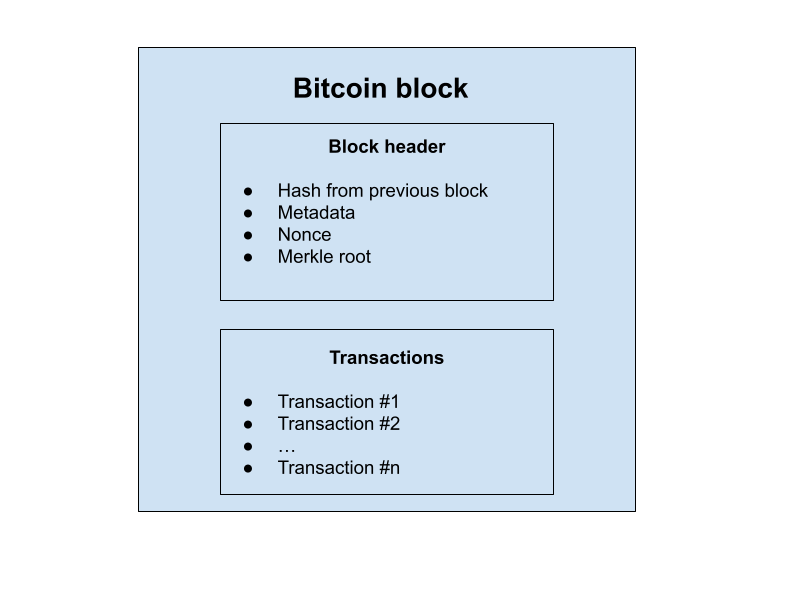
\includegraphics[width=130mm]{BitcoinBlock.png}
   \caption{Bitcoin block}
   \label{overflow}
   \end{figure}


\subsection{Proof-of-work}

A node must find a hash with a specific number of leading zeros to submit a new block.
The SHA-256 algorithm produces the hash, which is 256 bits long and typically represented as a 64-character hexadecimal string. 
The network's difficulty determines the number of leading zeros required, which sets the target value that the hash must be less than or equal to for the block to be valid.
For instance, the threshold might be $0000000000000000abc123...$
This cryptographic puzzle is a barrier to entry, ensuring that much computational power is spent creating the block.
The way to test different hash values is to change the block timestamp and the nonce value.
The nonce value is there solely for that purpose. Once a block is published, we cannot change any value inside of it because the hash value would change.
The immutability of the older blocks makes Bitcoin secure. To modify a block in the middle of the chain, we would need to redo the work of every block made after it.
The longest chain is determined by the cumulative proof-of-work invested in it. This is why we say that Bitcoin is secure as long as $51\%$ of the nodes are honest.
The chain with the majority of nodes working on it will grow the fastest and thus be the accepted chain.
The difficulty of the new block is determined by an average in order to generate blocks at a steady pace. A Bitcoin reward is also associated with mining (publishing) a block. \cite{MB17}


\subsection{Merkle Tree}
In the blockchain's architecture, only the Merkle root is stored in the block header. Nodes keep only the recent blocks in memory, and for older blocks, they keep only the block header.
This storage ensures the integrity of the blockchain while decreasing the memory required to have the full blockchain history.
Since the hash of a block is the hash of the block header, this strategy does not impact the integrity checks of the blockchain.
The Merkle root is the top of the Merkle tree and is a unique identifier of the full tree. A Merkle tree is a tree in which the parent node is the hash of the child nodes.
The tree is immutable because changing a single node would impact the Merkle root.


\iffalse
\begin{figure}[ht!]
 \centering
 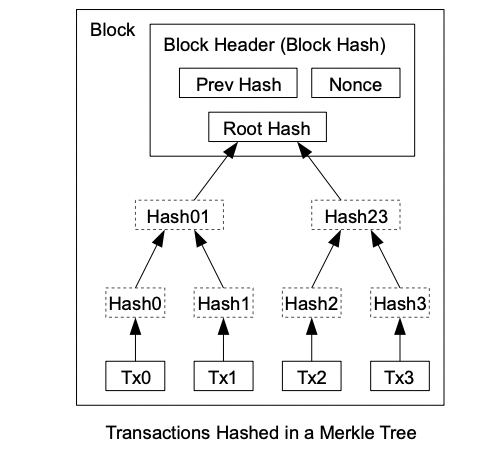
\includegraphics[width=90mm]{MerkleTree.png}
 \caption{Bitcoin Merkle Tree \cite{N08}}
 \label{overflow}
 \end{figure}
\fi


\section{Marketplaces}
The best way to buy Bitcoin for the first time is through marketplaces. Marketplaces facilitate the exchange of traditional currency for Bitcoin.
However, it's important to understand that the Bitcoin you purchase initially remains in the platform's custody rather than being sent directly to your personal wallet.
We need to request a transfer to our wallet to gain custody of our Bitcoin, similar to how traditional banking transactions rely on the bank to process our request.
Once we have Bitcoins in our wallet, we can transact on the network without needing a third party.
Unless we run a node, we must trust a third party, whether a marketplace or over-the-counter, to acquire Bitcoin first.

Since the Bitcoin ledger is public, we can use tools to view the network's transactions and to see which wallet address owns how many Bitcoins. 
When your Bitcoin is held in the marketplace's custody, it cannot be tracked onchain (onchain refers to everything happening in the blockchain). 
It blends with the plarform's holdings, because the marketplace does not have as many wallets as it has clients.
Marketplaces manage many wallets, some public and some private, which enhances the privacy of deposits and withdrawals but contradicts Bitcoin's design for transparency and independence from third parties. 
This lack of visibility poses a challenge, as users have no proof of the marketplace's solvency to reimburse all clients. 
However, this issue is being addressed through the introduction of proof of solvency (or proof of reserve) mechanisms, 
which allows marketplaces to demonstrate their solvency. 
While this is a positive development, current proof of solvency methods have shortcomings and are insufficient to prove solvency.


\section{Zero-Knowledge}
Zero-knowledge proof is a cryptographic technique allowing a prover to demonstrate knowledge of a fact without divulging additional information. 
For instance, rather than revealing the solution to an equation, zero-knowledge proofs enable the prover to show that they know the solution without revealing it. 
In this context, a witness is the secret information or evidence that supports the validity of the statement being proven. 
The goal is to construct a proof that is both sound and complete and is zero-knowledge \cite{LZK}.

\label{subsec:zkp}
\begin{itemize}
\item \textbf{Completeness}: If the statement is true, an honest verifier will be convinced by an honest prover.
\item \textbf{Soundness}: If the statement is false, no dishonest prover can convince the honest verifier (except with some infinitesimal probability).
\item \textbf{Zero-Knowledge}: If the statement is true,  a verifier learns nothing other than the statement is true. \cite{LC23}
\end{itemize}


\subsection{Non interactive proofs}

Zero-knowledge proofs were initially designed as interactive: multiple rounds of interaction between the prover and the verifier \cite{GMR89}.
Leading to what are called interactive zero-knowledge proofs. This interaction allows the prover to demonstrate knowledge of the solution without revealing additional information.
An alternative model was proposed in which the verifier and prover share a reference string during a trusted setup. Once we have the reference string, a single message is needed between the prover and the verifier.
Eliminating multiple rounds of interaction simplifies the verification process and reduces the computational power required.
Therefore, non-interactive zero-knowledge proofs offer enhanced efficiency and scalability, which will be needed later.  \cite{BFM88} \cite{GMW91}


\subsection{SNARKS}
One recent advance for non-interactive proofs is SNARK (Non-Interactive Argument of Knowledge).

This means a proof that is:
\begin{itemize}
\item \textbf{Succinct}: The proof size is minimal compared to the witness size (the secret information).
\item \textbf{Non-interactive}: There are no rounds of interactions between the prover and the verifier.
\item \textbf{Argument}: It is secure only against provers with bounded computational resources. A dishonest prover with unlimited computational power could potentially prove a false statement.
\item \textbf{Knowledge-sound}: A valid proof can only be generated if the prover knows the witness. \cite{NZ20}
\end{itemize}

Moreover, a SNARK can also be zero-knowledge, where the prover demonstrates knowledge without revealing additional information about the witness. We call such proof a zk-SNARK.
There are many techniques to construct a SNARK, but all of them follow the same guideline:
\begin{itemize}
   \item Express our problem as an arithmetic circuit
   \item Transform the circuit in a polynomial
   \item Commit the polynomial
   \item Interaction between the prover and the verifier to show that the polynomial solves the problem
 \end{itemize}

 We will show the core general idea behind a SNARK. 
We must transform the code we want to prove in a quadratic arithmetic program (QAP) to construct the SNARK.
The best example of a SNARK using this technique is Groth16\cite{GR16}, one of the most widely used SNARK today.


\subsubsection{Arithmetic circuit}
\label{subsec:ac}

Let us say we want to prove $x^3+x+5=35$.
The prover has to convince the verifier that he knows the solution without revealing it to him.

The first step in transforming a problem into the QAP form is to express it as an arithmetic circuit.
An arithmetic circuit is a set of gates, each assigned a distinct set of inputs corresponding to the numbers to be processed in the operation.
These gates are configured to execute arithmetic operations such as addition, subtraction, multiplication, or division. The outputs of the gate circuit represent the digits of the resulting computation.

\begin{figure}[H]
\centering
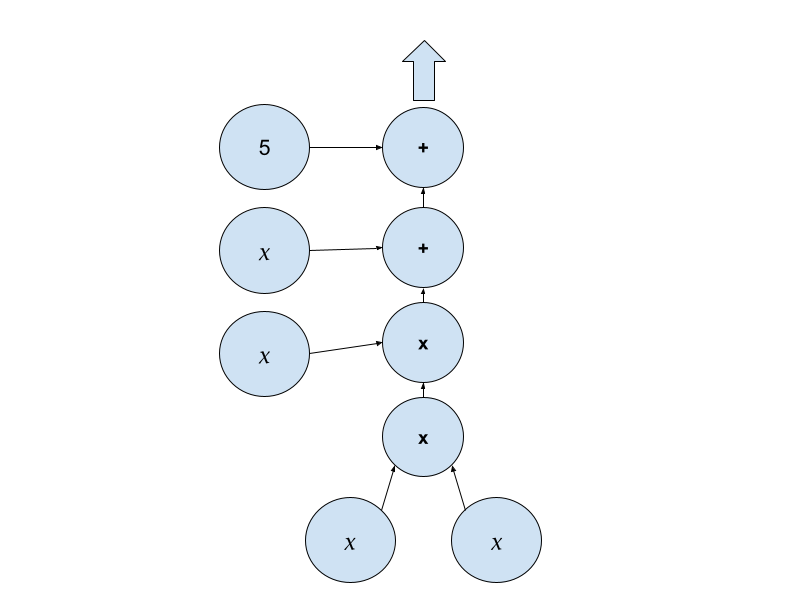
\includegraphics[width=130mm]{ArithmeticCircuit.png}
\caption{General Arithmetic circuit}
\label{overflow}
\end{figure}

\subsubsection{R1CS}
\label{subsec:r1cs}
The first step is to express our arithmetic circuit as a set of constraints where each constraint contains only one arithmetic operation.
\begin{quote}
$s_1 = x * x$
\\
$s_2 = s_1 * x$
\\
$s_3 = s_2 + x$
\\
$~out = s_3 + 5$
\end{quote}

We can now convert this into an R1CS.
An R1CS is a sequence of groups of three vectors $(a, b, c)$, where the solution to the R1CS is a vector $s$, and $s$ must satisfy the equation $s \cdot a * s \cdot b - s \cdot c = 0$, where $\cdot$ represents the dot product.
The length of each vector is the length of the total number of variables for the system. This includes a variable $one$ at the beginning, the variable $out$ at the end, and all intermediate variables.
The standard way of representing the three vectors $(a, b, c)$ is to create a mapping with the variables.
Here is the mapping we will use:
\\ 
$[one,out,x,s_1,s_2,s_3]$
\\
This gives us the first gate:
\begin{quote}
   $a = [0,0,1,0,0,0]$
   \\
   $b = [0,0,1,0,0,0]$
   \\
   $c = [0,0,0,1,0,0]$
\end{quote}
We are checking here that $x*x=s_1$.
$a$ and $b$ both represents $x$, while $c$ represents $s_1$.

 Let us verify that our first gate satisfies the solution equation:
   \\
   $s \cdot a * s \cdot b - s \cdot c = 0$
   \\
 We know that the solution to the equation is $ x = 3 $, so given that our $s$ vector
 would be: 
   \begin{quote}
   $s=[1,out,x,s_1,s_2,s_3]$
   \\
   $s=[1,35,3,9,27,30]$
\end{quote}

Now, if we do the dot product:
\begin{quote}
   $s \cdot a =  [1,35,3,9,27,30] \cdot [0,0,1,0,0,0] = 0*1+0*35+1*3+0*9+0*27+0*30= 3$ 
   $s \cdot b = [1,35,3,9,27,30] \cdot [0,0,1,0,0,0] = 3$ 
   $s \cdot c = [1,35,3,9,27,30] \cdot [0,0,0,1,0,0] = 9$ 
$s \cdot a * s \cdot b - s \cdot c =  3 * 3 - 9 = 0$

This shows that our solution vector satisfies the first gate.
\end{quote}

Following these rules, our second gate for $s_1*x=s_2$ is:
\begin{quote}
   $a = [0,0,0,1,0,0]$
   \\
   $b = [0,0,1,0,0,0]$
   \\
   $c = [0,0,0,0,1,0]$
\end{quote}

The third gate for $s_2+x=s_3$:
\begin{quote}
   $a = [0,0,1,0,1,0]$ ($s_2+x$)
   \\
   $b = [1,0,0,0,0,0]$ ($1$)
   \\
   $c = [0,0,0,0,0,1]$ ($s_3$)
\end{quote}

Fourth gate for $s_3+5=out$:
\begin{quote}
   $a = [5,0,0,0,0,1]$
   \\
   $b = [1,0,0,0,0,0]$
   \\
   $c = [0,1,0,0,0,0]$
\end{quote}

The R1CS put together:
\begin{quote}
   \[
 A =
   \begin{bmatrix}
      0 & 0 & 1 & 0 & 0 & 0 \\
      0 & 0 & 0 & 1 & 0 & 0 \\
      0 & 0 & 1 & 0 & 1 & 0 \\
      5 & 0 & 0 & 0 & 0 & 1
   \end{bmatrix}
   \]
   \[
 B =
   \begin{bmatrix}
      0 & 0 & 1 & 0 & 0 & 0 \\
      0 & 0 & 1 & 0 & 0 & 0 \\
      1 & 0 & 0 & 0 & 0 & 0 \\
      1 & 0 & 0 & 0 & 0 & 0
   \end{bmatrix}
   \]
   \[
 C =
   \begin{bmatrix}
      0 & 0 & 0 & 1 & 0 & 0 \\
      0 & 0 & 0 & 0 & 1 & 0 \\
      0 & 0 & 0 & 0 & 0 & 1 \\
      0 & 1 & 0 & 0 & 0 & 0
   \end{bmatrix}
   \]
   \end{quote}
   
\cite{RC23}


\subsubsection{QAP}
The next step is converting our R1CS into QAP form, which uses polynomials instead of dot products.
We do this by using polynomials instead of a dot product.
In order to get a polynomial, we need to do a Lagrange interpolation on a set of points.
For a polynomial of degree $n$, we need $n+1$ set points for the interpolation to give the polynomial.
We need a polynomial of degree $n$, where $n$ is the number of rows $- 1$. (Same thing as the number of gates $-1$). 
Therefore, we need a set of 4 points to have a polynomial.
We can get 18 ($3*6$) polynomials by transposing our matrices.
For instance, the first column of $A^T$ is our first polynomial $[0,0,0,5]$.
This gives us the set of points $[(1,0),(2,0),(3,0),(4,5)]$.
The polynomial interpretation of this set of points is $f(x) = 535x^3+636x^2+116x+636$.
Doing the same for every column of $A$, $B$ and $C$, we get the matrices:
\begin{quote}
   \[
 A_m =
   \begin{bmatrix}
      636 & 116 & 636 & 535 \\
      0   & 0   & 0   & 0   \\
      8   & 416 & 5   & 213 \\
      635 & 330 & 637 & 321 \\
      4   & 634 & 324 & 320 \\
      640 & 536 & 640 & 107
   \end{bmatrix}
   \]
   \[
 B_m =
   \begin{bmatrix}
      3   & 529 & 323 & 427 \\
      0   & 0   & 0   & 0   \\
      639 & 112 & 318 & 214 \\
      0   & 0   & 0   & 0   \\
      0   & 0   & 0   & 0   \\
      0   & 0   & 0   & 0
   \end{bmatrix}
   \]
   \[
 C_m =
   \begin{bmatrix}
      0   & 0   & 0   & 0   \\
      640 & 536 & 640 & 107 \\
      0   & 0   & 0   & 0   \\
      4   & 423 & 322 & 534 \\
      635 & 330 & 637 & 321 \\
      4   & 634 & 324 & 320
   \end{bmatrix}
   \]
   \end{quote}
   
The polynomial we obtained from the first column of $A$ appears in the first row of $A_m$. We obtained each row similarly.

The point of this transformation is that the dot product is now a series of additions and multiplications of polynomials, and the result will be a polynomial.

The resulting polynomial needs to equal $0$ at all the $x$ coordinates we used previously.
If it does, it means that the checks pass.
We do not need to evaluate our polynomial at every point to verify correctness. 
We can instead divide our polynomial $t$ by another polynomial $z$ and verify that the division leaves no remainder.
We define $Z$ as $(x - 1) * (x - 2) * (x - 3) * ...$, the simplest polynomial that is equal to zero at all points that correspond to logic gates. 

In this case, computing T:
\begin{quote}
$T(x) = S \cdot A_m * S \cdot B_m - S \cdot C_m  $

$T(x) = 139*x^6 + 372*x^5 + 275*x^4 + 58*x^3 + 147*x^2 + 379*x + 553$
\end{quote}

In this case, we use $Z = (x-1)(x-2)(x-3)(x-4)$
To show that $T$ is divided by $Z$, it is sufficient to verify $T(x) = 0$ at $1,2,3$ and $4$.

More formally, we have shown that there exists a Polynomial $H$ such that $T(x)=H(x) \cdot Z(x)$
(i.e. if $T$ is divided by $Z$, then it will be perfectly divisible and will leave no remainder)


Groth16 is an all-in-one zkSNARK, meaning the polynomial commitment scheme is included in the design. Other SNARK desings such as Plonk and Marlin.
In a zkSNARK, the prover demonstrates that a polynomial $Z$ exactly divides another polynomial
$T$ using Polynomial Commitments, such as KZG, Bulletproofs, or FRI. 
The purpose of this step is to reveal only certain evaluations of the polynomial without disclosing the entire polynomial itself.\cite{VB16}


\subsection{Polynomial Commitments}
\label{subsec:pc}
A polynomial commitment is a cryptographic technique that allows one to commit to (or "lock") a polynomial's data 
in such a way that the data can later be revealed (or "unlocked") while ensuring integrity and privacy.

Polynomial commitments are binding, meaning that once a commitment is made, it is computationally infeasible to alter the original polynomial without detection. 
The commitments are generally of constant size. While collisions are theoretically possible due to the pigeonhole principle, finding a second polynomial that matches the same commitment is computationally infeasible.

Additionally, polynomial commitments can be hiding, which means the verifier is not exposed to any information about the polynomial.
For example, we can create a commitment by hashing a polynomial with a collision-resistant hash function like SHA-256, and only the hash value is shared. 
To make it hiding, a random factor could be added to the polynomial data before hashing.

Instead of committing to an entire dataset (a set of values or a table), we can commit to a polynomial representing or encoding this data. 
This is useful because polynomials can be compact representations of structured data.

The naïve approach to committing to a polynomial is simply revealing its coefficients directly.
This approach fails because the information is not hidden, among other things.

A well-designed polynomial commitment scheme allows flexibility: it enables someone to either open the commitment to reveal the entire polynomial or to open it at a specific evaluation point. 
This is a necessary parameter of the scheme, as it allows verification that someone knows a polynomial that evaluates at a certain point without revealing the polynomial itself.

For the proof to be complete, the polynomial must be evaluated at $d+1$ unique points, where $d$ is the degree of the polynomial.
However, to be succinct, we want to verify the least number of points possible.

How many points do we need to verify to have a high confidence in the polynomial?
In a cryptographic setting, $q$ is a large prime. If $q$ is 256-bits and the polynomial is degree 1000, 
then the probability of giving the correct value at random is $1000/2^{256}$ (As we recall, a polynomial of degree 1000 has 1000 roots). 
Therefore, after checking just one random point, it is statistically probable that the polynomials will be the same if the point matches. \cite{VR23}

Many different polynomial schemes exist, such as KZG, Bulletproofs and FRI. 
In these schemes, the setup processes and the commitments vary significantly. 

KZG commitments rely on a trusted setup to generate elliptic curve parameters\cite{KZG}. The KZG setup is universal. Once it is done, it can be useable by anyone. 
Many different versions are available to the public; the Ethereum Foundation has implemented one of these versions. 

Bulletproofs avoids using a trusted setup by using logarithm-based techniques\cite{BP18}. 
However, while the KZG proofs are constant size, Bulletproofs are logarithmic.

FRI evaluates polynomials through proximity checks.\cite{FRI} FRI is post-quantum since it relies only on hash function security. 
Other schemes rely on cryptographic assumptions, such as the hardness of the discrete logarithm problem, which quantum computers can efficiently solve.


\subsubsection{KZG}
KZG commitments work by evaluating the polynomial at a single secret point $\tau$. 
As we just saw, evaluating a single point is statistically sufficient.
This approach ensures that the commitment remains succinct.

To achieve this, a trusted setup generates a structured random string (SRS) containing powers of $\tau$
of a specific polynomial degree. 
\[
\langle g^{\tau^0}, g^{\tau^1}, g^{\tau^2}, g^{\tau^3}, \dots, g^{\tau^d} \rangle \equiv \text{SRS}
\]
where \( g \) is a generator.  
The prover uses these precomputed values to commit to \( f(x) \) without knowing \( \tau \) or \( P(\tau) \).

\begin{equation*}
 K_P(\tau) = \text{Commit}(P(\tau))
\end{equation*}
\begin{equation*}
 = g^{c_0} (g^\tau)^{c_1} (g^{\tau^2})^{c_2} (g^{\tau^3})^{c_3} \dots
\end{equation*}
\begin{equation*}
 = g^{c_0 + c_1 \tau + c_2 \tau^2 + c_3 \tau^3 + \dots}
\end{equation*}
\begin{equation*}
 = g^{P(\tau)}
\end{equation*}

The commitment is succinct because the polynomial degree does not impact the size.


The prover can send the coefficients to open the polynomial, and the verifier will recompute $K_P(\tau)$.
This is of little use since the prover could have hash the coefficient to get a similar result.
KZG offers additional features that work specifically with polynomials.

Additive homomorphism in KZG allows commitments of polynomials to be combined in a way that reflects polynomial addition. 
If two polynomials $f$ and $g$ have a sum $f + g = h$, then their commitments $C_f$ and $C_g$ have the sum $C_f + C_g = C_h$.

Multiplication is not exactly homomorphic in KZG, but we can get something close to it using bilinear pairing.
The idea is to assert the value for $K_{P_1(\tau)} \cdot K_{P_2(\tau)}$ and convince it is correct given $K_{P_1(\tau)}$ and $K_{P_2(\tau)}$.

\begin{quote}
   \begin{equation*}
 e(K_{P_1(\tau)}, K_{P_2(\tau)}) \stackrel{?}{=} e(K_{P_1(\tau) + P_2(\tau)}, g)
   \end{equation*}
   \begin{equation*}
 e(g^{P_1(\tau)}, g^{P_2(\tau)}) = e(g^{P_1(\tau) \cdot P_2(\tau)}, g)
   \end{equation*}
   \begin{equation*}
 = e(g, g)^{P_1(\tau) \cdot P_2(\tau)}
   \end{equation*}
\end{quote}
   


The most beneficial property of KZG and any polynomial commitment scheme is the ability to open the commitment at specific points.

KZG commitments allow proving that a polynomial \( P(x) \) has a root at \( r \) by demonstrating that \( (x - r) \) divides \( P(x) \) without remainder.
As we recall, we can write any polynomial in a factorized format:

$P(x) = (x - r_0)(x - r_1)(x - r_2) \dots$

If \( r \) is a root, \( P(x) \) is divisible by \( (x - r) \), so we define:

$Q(x) = \frac{P(x)}{x - r}$

The prover commits to \( K_{Q(\tau)} \) and provides it to the verifier.

The verifier can compute $K_{V(\tau)}$ by treating $x-r$ as a polynomial:

$V(x) = x - r = -r + 1 * x$
and using KZG to produce it.
\begin{quote}
   \begin{equation*}
 e(K_{P(\tau)}, g) \stackrel{?}{=} e(K_{Q(\tau)}, K_{V(\tau)})
   \end{equation*}
   \begin{equation*}
 e(g^{P(\tau)}, g) = e(g^{Q(\tau)}, g^{V(\tau)})
   \end{equation*}
   \begin{equation*}
 e(g, g)^{P(\tau)} = e(g, g)^{Q(\tau) \cdot V(\tau)}
   \end{equation*}
\end{quote}


This proof is independent of the polynomial degree of $Q$ and $P$, making it efficient even for large polynomials.


The security of the commitments relies on properly generating the trusted setup. 
If the secret $\tau$ is leaked or manipulated, the security of the scheme could be compromised. 
To mitigate this, multi-party computation ceremonies ensure that at least one participant securely destroys their contribution to the SRS. 
Zero-knowledge proofs can validate that the setup was generated correctly without revealing $\tau$.

KZG is the standard in terms of commitments for SNARKS. It is efficient and forms the basis of many cryptographic protocols. \cite{vODC24}


\section{Proof of solvency}

A proof of solvency is a system where we prove that an entity, in most cases an exchange, holds enough assets to cover
the balance of every customer. In traditional finance, this would be done through an audit. While an audit can be helpful,
it has many limitations. It requires the trust of another third party, but it also poses a time constraint. Thus, it is impractical, even impossible, to hold an audit daily, and things move fast in the Bitcoin world. It is essential to be able to fill a proof of solvency every single day.
Therefore, implementing a mechanism to produce daily proof of solvency is of the utmost importance.

A proof of solvency is composed of a proof of assets, where we verify what assets the marketplace has control over, and the proof of liabilities, 
where we confirm that the total amount of user deposits is smaller than the sum of the marketplace's assets.

The first paper about a proof of solvency focuses only on the proof of liabilities. In his paper, Gregory Maxwell addresses the issue of verifying
the solvency of Bitcoin exchanges. \cite{chainlink_blog}
Maxwell's system ensures user privacy by maintaining the confidentiality of individual account balances while only revealing aggregate information in the proof of liabilities.
This is achieved through the application of Merkle trees.


\begin{figure}[H]
\centering
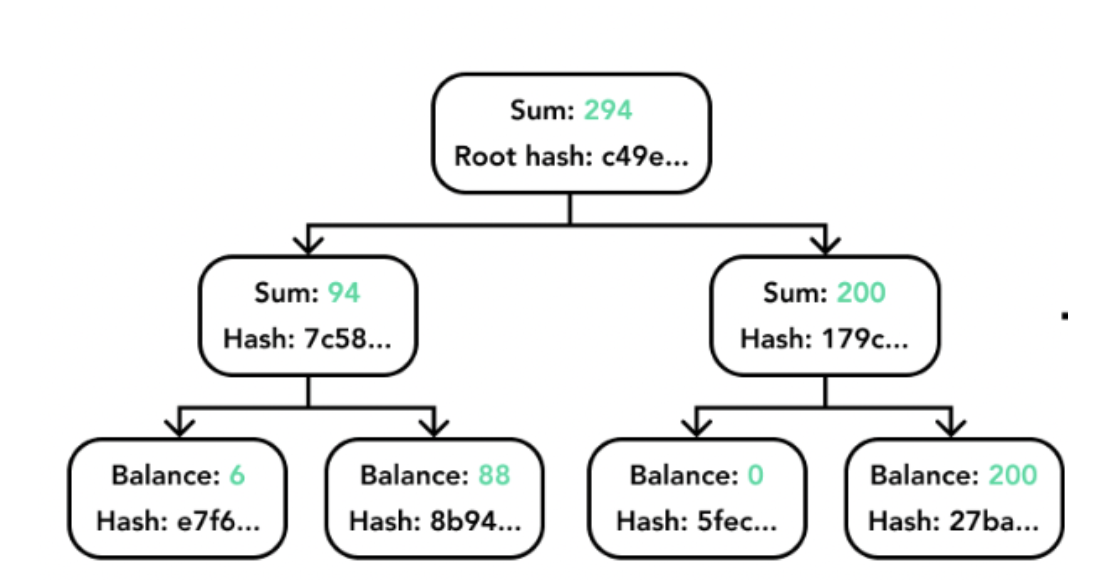
\includegraphics[width=130mm]{MerkleTreeLiabilities.png}
\caption{Merkle tree for proof of liabilities}
\label{overflow}
\end{figure}


In the Merkle tree, every node contains a user's balance and a hash-based commitment incorporating the customer ID and a nonce. The root of the tree is the sum of the balances.
Users receive a subset of the hash tree from the exchange to verify their inclusion in the total liabilities. This subset includes the user's nonce and the sibling nodes along the unique path from the user's leaf node to the root.
Users can confirm the inclusion of their balance by comparing the received information to the exchange's broadcasted root node.
While elegant, the protocol does have privacy implications. The exact value of the exchange's total liabilities, published in the root node, may be sensitive data.
Additionally, the proof of inclusion reveals the neighbor's balance and the subtree's balance along the Merkle path.

The proof of liabilities is only part of the proof of solvency. A complete proof of solvency needs a proof of asset as well.
Provision describes the first preserving privacy proof of asset \cite{DBBBCC15}.

In Provisions, the focus shifts toward preserving privacy while still proving ownership of assets.
Instead of publicly demonstrating control over specific addresses, Provisions enables exchanges to prove ownership of an anonymous subset of addresses sourced from the blockchain.

Since these 2 papers, a lot of work has been done to evolve the proof of solvency. However, marketplaces still do not implement a proof of solvency or a flawed and limited version of it.


\subsection{Real world proof of solvency}
In recent years, several major cryptocurrency exchanges, including Binance, Crypto.com, and Kraken, have taken steps to enhance transparency by providing various proof of reserves.
Binance has implemented a proof of reserves system where they publish a monthly Merkle tree as their proof of liabilities and disclose a list of their assets (every cryptocurrency under their control) \cite{BPR}.
Crypto.com published a one-time audit \cite{CC22}.
Kraken also publishes proof of liabilities every few months without proof of assets. \cite{KK23}.

Although these proof of reserves may seem promising initially, they are primarily superficial.
The proofs have many shortcomings; they are insufficient to prove that the marketplaces are solvent.
The first concern is the lack of proof of assets, or in Binance's case, the lack of evidence demonstrating control over the wallets.
Without reliable proof of assets, the proof of liabilities is worthless because it has nothing to compare against.

Moreover, the frequency of reporting is another area of concern. Given the dynamic nature of cryptocurrencies, a monthly report is not sufficient.
Binance is the only marketplace describing its proof of solvency, and we can see that it is not built with recurrence in mind.
The proof is created from scratch every time. They would need 150 servers to produce a daily proof \cite{BPS}.

